\chapter{Onde tridimensionali}
\lecture{12}{4 aprile 2024}

Per ora abbiamo lavorato sempre con onde unidimensionali \(\xi (x,t)\), per i mezzi non dispersivi l'equazione di riferimento è l'equazione di D'Alembert:
\begin{equation}\label{eq:dalembert}
	\frac{\partial ^{2} \xi }{\partial ^{2} x^{2} }= \frac{1}{v^{2} }\frac{\partial ^{2} \xi }{\partial t ^{2} }  
\end{equation}
dove \(v\) rappresenta la velocità dell'onda (che per le onde armoniche è uguale alla velocità di fase e anche alla velocità di gruppo).
Per estendere la trattazione allo spazio tridimensionale dovremo passare da due a quattro variabili: \((x,y,z,t)\) o \(\vec{r} , t\).
\section{Equazione di D'Alembert tridimensionale}
Procederemo per maniera euristica. Ricordiamo il significato dei termini nell'equazione \eqref{eq:dalembert}: il membro di sinistra rappresenta una differenza di tensioni ai lati dell'elemento infinitesimo di corda, mentre il membro di destra rappresenta l'accelerazione verticale della corda. È naturale provare a modificare il membro di sinistra per poter tenere conto di tutte le direzioni da cui possono provenire le forze:
\begin{figure}[H]
	\centering
	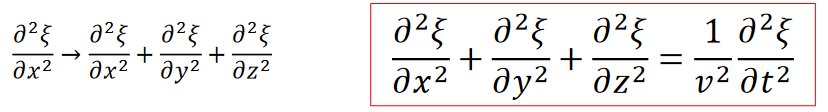
\includegraphics[width=0.7\textwidth]{screenshots/2024-04-04-09-31-11.png}
\end{figure}
che può essere riscritta semplicemente utilizzando il laplaciano:
\begin{equation} \label{eq:dalembert3d}
	\laplacian{\xi (\vec{r} , t)}= \frac{1}{v^{2} }\frac{\partial ^{2} \xi }{\partial t ^{2} } 
\end{equation}
Questa equazione ha diverse proprietà già viste per l'equazione in una dimensione:
\begin{itemize}
	\item È omogenea, quindi la soluzione banale è sempre presente: \(\xi (\vec{r} , t)=0\).
	\item È lineare ed è associata a un operatore molto importante: l'operatore di D'Alembert o \emph{d'Alambertiano}
	\[
		\hat{L} = \left( \laplacian - \frac{1}{v^{2} }\frac{\partial ^{2} }{\partial t ^{2} }  \right) \to \hat{L} (\xi (\vec{r} , t))=0
	\]
	L'equazione appena scritta può essere rappresentata più semplicemente con \(\Box \xi (\vec{r} , t) = 0\).	
	\item Vale il principio di sovrapposizione.
\end{itemize}
Si nota immediatamente che il caso unidimensionale è un caso limite dell'equazione \eqref{eq:dalembert3d} in cui \(\xi (\vec{r} , t)\) dipende esclusivamente da \(x\). L'unica differenza è che in questo caso l'onda è definita in tutto lo spazio e non solo sull'asse \(x\).

\paragraph{Soluzioni dell'equazione}
Al contrario del caso unidimensionale, in tre dimensioni abbiamo due soluzioni (una per ciascun verso di propagazione) per ogni direzione disponibile dello spazio. In altre parole, \(\forall \hat{\vec{u}}, \forall f,g \in \mathcal{C} ^{2}  \), \(\xi (\hat{\vec{u}} \cdot \vec{r} - vt )\) e \(\xi (\vec{r} , t)= g(\hat{\vec{u}} \cdot \vec{r} + vt)\) sono soluzioni.
\begin{proof}
	Poniamo \(s=\hat{\vec{u}} \cdot \vec{r} - vt \), \(\xi (\vec{r}, t)=f(s)\).
	\begin{figure}[H]
		\centering
		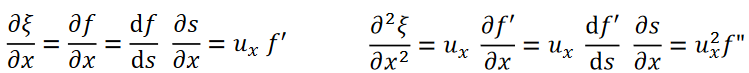
\includegraphics[width=0.6\textwidth]{screenshots/2024-04-04-09-47-49.png}
	\end{figure}
	Di conseguenza, \(\laplacian{\xi } \) diventa:
	\begin{figure}[H]
		\centering
		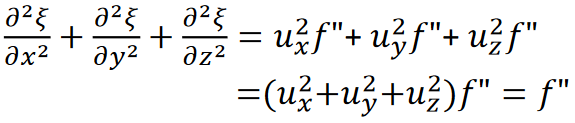
\includegraphics[width=0.5\textwidth]{screenshots/2024-04-04-09-49-05.png}
	\end{figure}
	E come nel caso unidimensionale,
	\[
		\frac{1}{v^{2} }\frac{\partial ^{2} \xi }{\partial t^{2} } = \frac{1}{v^{2} } v^{2} f^{\prime\prime} = f^{\prime\prime} 
	\]
	L'unico aspetto che conta ai fini della dimostrazione è che \(f^{\prime\prime} \) esista! Quindi \(f(\hat{\vec{u}} \cdot \vec{r} - vt)\) è una soluzione dell'equazione di D'Alembert. Più precisamente è un'onda progressiva nella direzione e verso individuata da \(\hat{\vec{u}}\).
\end{proof}

\paragraph{Cerchiamo il conforto del passato}
Quando \(\hat{\vec{u}} \equiv \hat{\vec{i}} \), \(\hat{\vec{u}} \cdot \vec{r} = x \rightsquigarrow \xi (\vec{r},t ) = f(x-vt) = \xi (x,t)\), che è l'onda progressiva in una dimensione già conosciuta ma che si muove nella direzione delle \(x\) positive, con la differenza, come detto prima, che questa volta l'onda occupa tutto lo spazio.

\paragraph{Struttura delle onde}
Consideriamo per ora onde con \(u_z = 0\), \(\hat{\vec{u}} \equiv u_x \hat{\vec{i}} + u_y \hat{\vec{j}} \rightsquigarrow \hat{\vec{u}} \cdot \vec{r}\). Consideriamo un'onda impulsiva con un solo massimo in \(s=0\).
\begin{figure}[H]
	\centering
	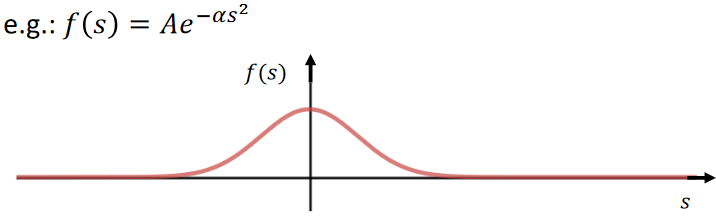
\includegraphics[width=0.6\textwidth]{screenshots/2024-04-04-09-56-08.png}
\end{figure}
Studiamo il moto del massimo dell'onda: \(s=xu_x + yu_y - vt = 0 \rightsquigarrow xu_x + yu_y = vt\).
\begin{figure}[H]
	\centering
	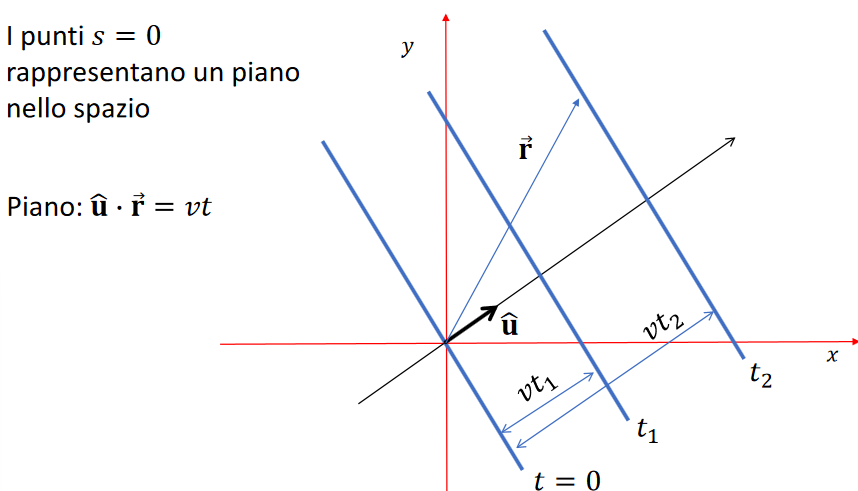
\includegraphics[width=0.7\textwidth]{screenshots/2024-04-04-09-57-56.png}
	\caption{La retta blu va immaginata come un piano in tre dimensioni perpendicolare alla direzione individuata dal versore \(\hat{\vec{u}} \) che si muove con velocità \(v\).}
\end{figure}
% TODO: recupera definizione fronti d'onda
Queste onde sono dette onde piane, sembra che serva un piano infinito per generarle! In realtà sono generalmente impiegate come approssimazione di onde reali che altrimenti non sarebbero piane (quindi in una zona piccola lontana dalla sorgente).

\paragraph{Onde armoniche piane}
Nel caso tridimensionale un'onda armonica può essere scritta come \(\xi (\vec{r},t ) = A \cos (k \hat{\vec{u}} \cdot \vec{r} - \omega t)\). Questa è detta onda armonica piana.
\begin{definition}
	[Vettore d'onda]
	\[
		\vec{k} = k \hat{\vec{u}} 
	\]
	\(\vec{k}\) individua la direzione di moto dell'onda e il suo modulo è il numero d'onda \(k\). \(\vec{k}\) è quindi perpendicolare ai fronti d'onda.
\end{definition}
% TODO: recupera serie di Fourier L18 per onde tridimensionali